{
\newcommand{\figWidtha}{8.cm}
\newcommand{\figWidthb}{10.cm}
\newcommand{\trimfiga}[2]{\trimPlotb{#1}{#2}{.0}{.0}{.0}{.0}}
\newcommand{\trimfigb}[2]{\trimPlotb{#1}{#2}{.05}{.1}{.05}{.1}}
\begin{figure}[hbt]
 \begin{center}
%
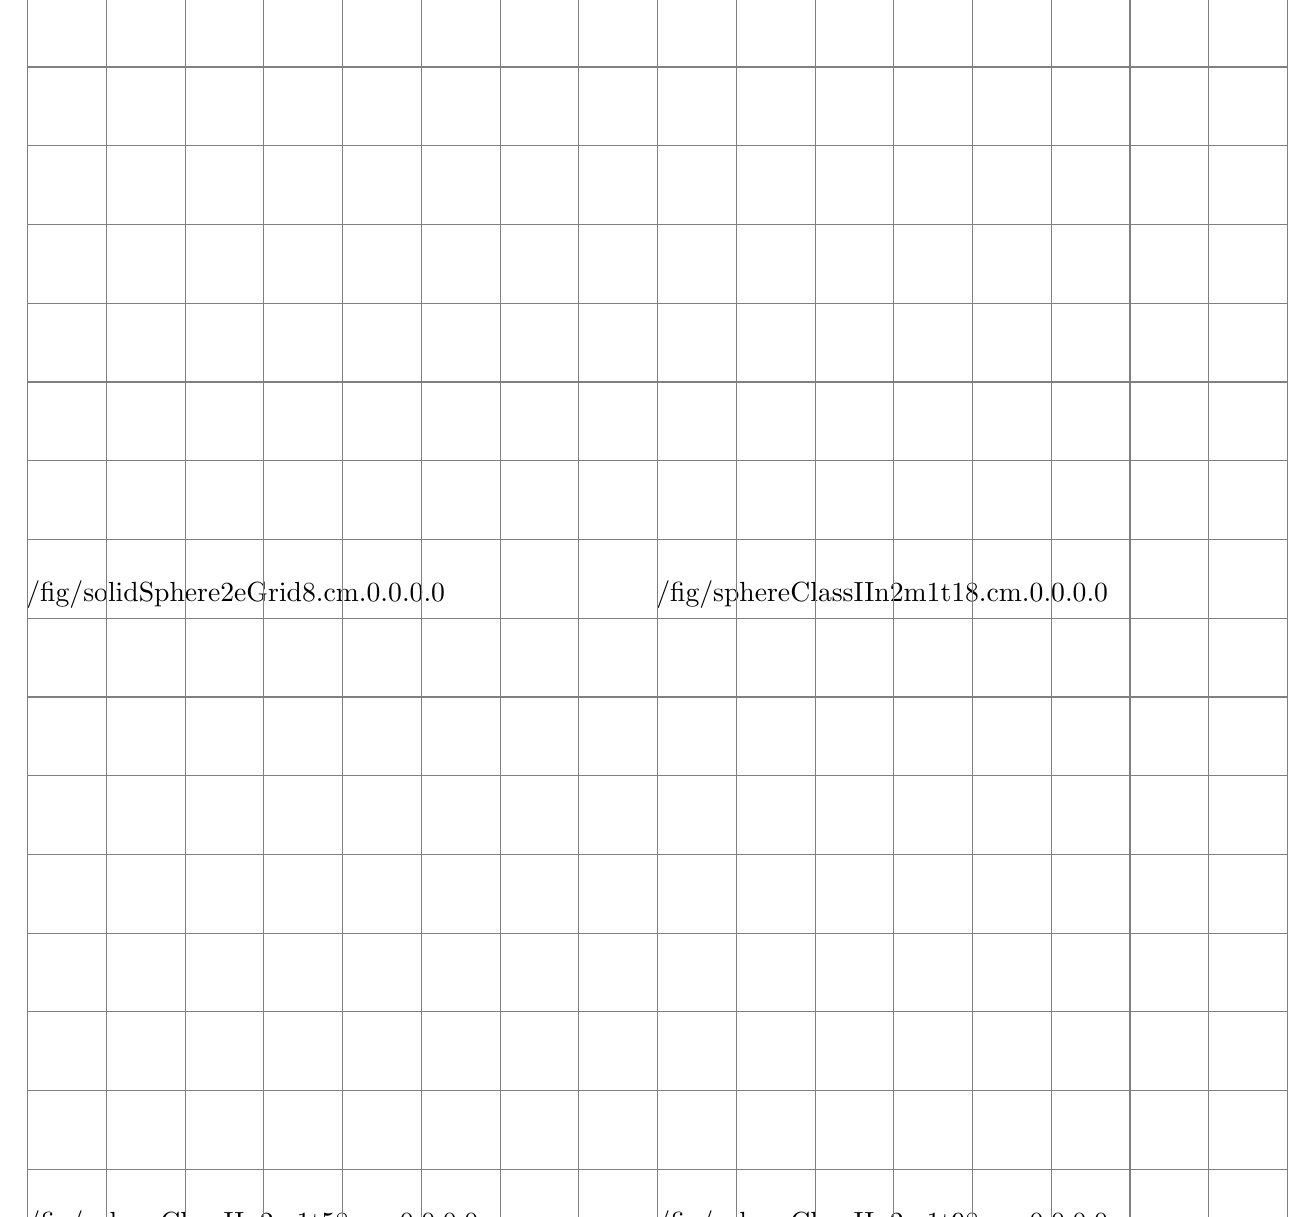
\begin{tikzpicture}[scale=1]
  \useasboundingbox (0,.75) rectangle (16.,15.5);  % set the bounding box (so we have less surrounding white spa  
  \draw ( 0.0,8.0) node[anchor=south west,xshift=-4pt,yshift=+0pt] {\trimfiga{\smDocDir/fig/solidSphere2eGrid}{\figWidtha}};
  \draw ( 8.0,8.0) node[anchor=south west,xshift=-4pt,yshift=+0pt] {\trimfiga{\smDocDir/fig/sphereClassIIn2m1t1}{\figWidtha}};
  \draw ( 0.0,0.0) node[anchor=south west,xshift=-4pt,yshift=+0pt] {\trimfiga{\smDocDir/fig/sphereClassIIn2m1t5}{\figWidtha}};
  \draw ( 8.0,0.0) node[anchor=south west,xshift=-4pt,yshift=+0pt] {\trimfiga{\smDocDir/fig/sphereClassIIn2m1t9}{\figWidtha}};
% grid:
  \draw[step=1cm,gray] (0,0) grid (16,16.);
\end{tikzpicture}
\end{center}
\caption{Vibrational mode of an elastic sphere. Left: overlapping grid for a
solid sphere consisting of two orthographic patches, a spherical polar shell and
an interior Cartesian grid (not visible). Middle to right: the deformed sphere at times $t=0$, $t=0.8$ 
and $t=1.2$ for the case $\rho=\lambda=\mu=1$ and $R=1$.  The displacement is scaled by a factor of $0.08$ for illustrative purposes.}
\label{fig:sphereEigEvolution}
\end{figure}
}


